\chapter[
Capacitive Load Cells to 
 Promote Worker Safety
]{
Low-Profile Capacitive Load Cells for 
 Underground Mining Material and Wear Classification
 to Promote Worker Safety
\label{chap:P1}
}

\newcommand{\ora}{\overrightarrow}

\begin{center}
This article has been published open access and is part of the public domain.
The copyright remains property of the author.
\end{center}

\subsection{Abstract}

This work proposes a capacitive load cell for conical picks to enable 
 underground continuous mining machine operators to 
 perform their roles away from known hazardous regions near the machine.
The load cell is embedded in commercially available flexible printed circuit board,
 integrates with the target tooling, and demonstrates in-situ force sensing 
 of vibration signatures for continuous mining cutting tools.
Changes in material constitution, tool mass, and tool geometry cause modal variations
 in vibrational response measurable with force sensors at the cutting interface.
Time-series measurements are captured during rock cutting tests using a linear cutting machine.
These measurements are segmented into small windows, less than 0.25 seconds, and are preprocessed 
 using the fast Fourier transform, which highlights the modal variations.
The transformed measurements are then classified into different material and wear categories
 using support-vector machines with the radial basis function kernel.
Different normalization schemes and Fourier transform methods are tested for signal preprocessing.
Results show that the power spectral density measurements with normally distributed coefficients 
 give good results for material classification, while the normalized time-domain measurements
 give better results for wear classification.
Under laboratory conditions, this technique is shown to 
 classify material and wear categories with F1 score above 0.85 out of 1.0 for our experiment.
This technology could be used to assist operators in assessing material and wear conditions from
 a safer distance. 
It has applications in the coal mining industry as well as other applications
which use conical picks such as road milling.

\subsection{Introduction}\label{sec1}

Operators monitoring important process feedback in hazardous regions is dangerous \cite{jobes12}.
Operators are expected to monitor machine alignment, tool wear, machine condition, and the material being cut \cite{sanders81}.
The hazards that the operators are exposed to in underground mining can be difficult to model \cite{JiangYaodong2017Arom}.
To allow operators to perform their role from a greater distance, 
 we propose a sensor suitable for assisting operators in assessing material type and tool wear that integrates
 with conical picks on continuous miners used in underground coal mining.

Underground mining is dangerous and safety has not been improved over the last decade, 
 with fatalities per 100,000 full time equivalent employees averaging 21.4 from 2011-2020 \cite{nioshdata}.
In particular, coal workers are roughly 50\%
 more likely to be injured than workers in other mining sectors and
 account for roughly 50\% of fatalities from 1983 to 2020\cite{nioshdata}.
Existing technologies for mitigating these hazards monitor the environment 
 with micro-seismic sensors, distributed pressure sensors, or electromagnetic analysis \cite{JiangYaodong2017Arom}.
These technologies only identify hazards after they occur. 
Elimination of hazardous conditions is the most effective method for reducing risk to workers in any application \cite{niosh_2015}.
The only way to eliminate these hazardous conditions is to allow the operators to perform their role from a greater distance.

Previous efforts to allow operators to perform their role from a greater distance,
 namely development of remote controls, have allowed operators to 
 collect better visual feedback; however, 
 operators often put themselves in hazardous positions to do so \cite{bartels09}.
Technologies also assist operators by automating some tasks. 
For example, automated hydraulic diagnostic systems can help operators 
 monitor the machine's hydraulic conditions \cite{mitchell91}.
One of the most effective technologies for reducing worker injury is the personnel proximity detector, 
 which disables certain machine operations if designated zones near the machine are entered 
 by persons tracked with the device \cite{bissert16}. 
This device was implemented about a decade ago; however, there have not been 
 any major improvements since.

Direct measurements of rock and pick interaction have previously noted 
 significant differences in forces between tool wear levels \cite{sundae85, donna90}.
Material has been differentiated by vibration signatures using various classification techniques
 as early as 1993 \cite{gary93}.
Previous efforts for smart bit or intelligent pick tooling to perform these tasks in real-time during operation 
 have taken place over the last few decades, examples include:
 using neural networks to classify tool wear in potash \cite{potashMeyersThesis}, 
 using acoustic data to classify both material and tool wear in coal cutting \cite{shen1996acoustic}, 
 using piezo sensors to deduce rock chipping \cite{smartbitMillerThesis},
 and, most recently, using an instrumented block with integrated strain gauges to measure cutting forces \cite{fries21}.
So far, results using capacitive load cells have not been found for 
 material and tool wear classification in underground mining. 
Advances in both capacitive sensing and vibration classification 
 have unearthed a variety of applications in other domains.
Our sensor, shown in Fig.~\ref{fig:senseonpick}, can assist operators in assessing material type and tool wear
 by measuring differences in vibrational responses between the different conditions.


\begin{figure}[t!]
\centering
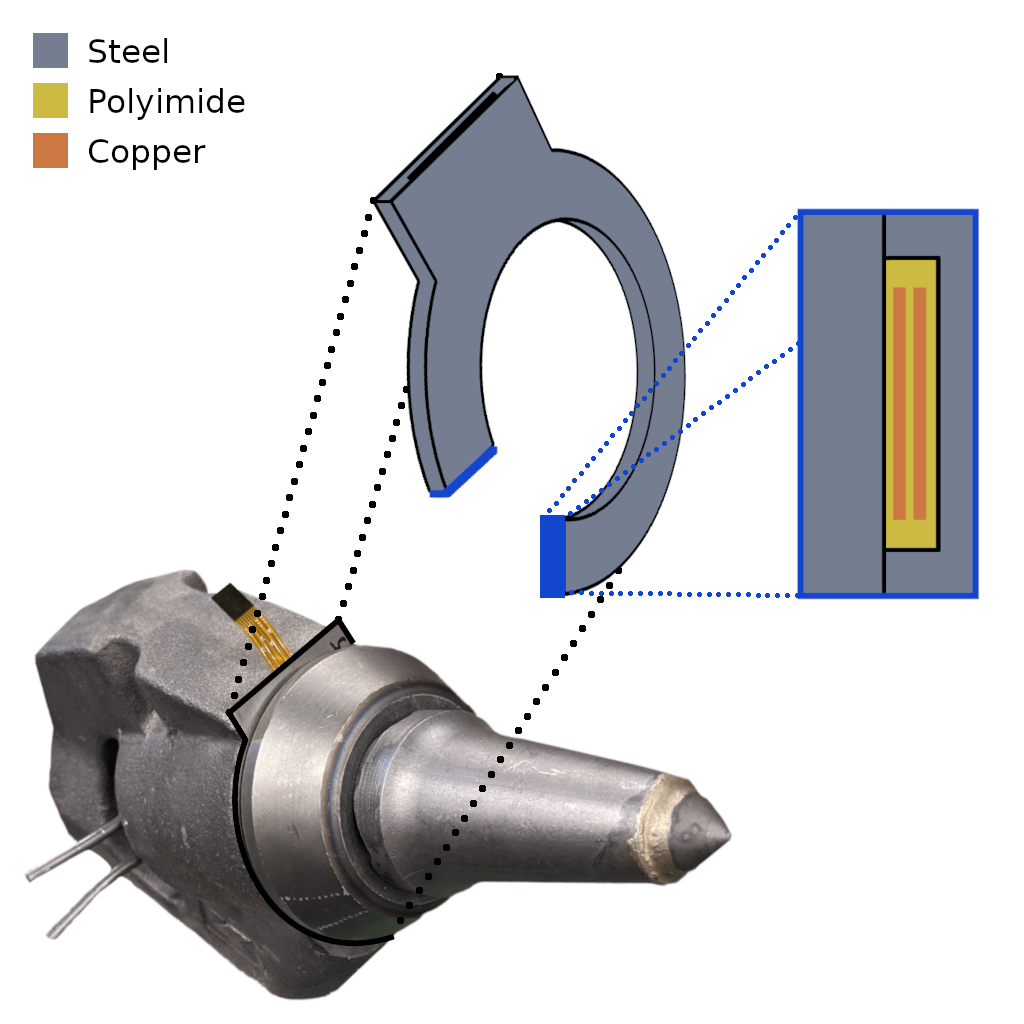
\includegraphics[width=3in]{figures/p1_media/Fig1.png}
\caption{A prototype of the sensor integrated with the U92 4.0 22NB  Conical Pick
 and K35 Block system, from Kennametal. The device is shown without the measurement
 collection system and is situated between the sleeve and the block.
The FlexPCB interface is exposed, which provides access to the capacitive sensors' electrodes.
 A steel case protects the FlexPCB sensor and
provides the necessary stiffness to transfer the input forces to the sensor.
An embedded electronics platform, not shown in this figure, takes measurements
 suitable for dynamic classification of tool-wear and material. 
A cutaway of the sensor shows the thin film design for the force sensor.}
\label{fig:senseonpick}
\end{figure}


To test our sensor for material and wear classification, full-scale rock cutting experiments are 
 performed using the linear cutting machine at Colorado School of Mines,
 a popular type of tool for rock cutting mechanics testing \cite{rostami21}.
A limestone sample cast in concrete is used to test material classification. 
Conical picks of three different wear levels at an attack angle of 45 degrees are used for tool wear classification.
The wear levels are \textit{new}, \textit{moderate}, and \textit{worn}, where \textit{moderate}
 represents a pick halfway through its useful life, and \textit{worn} is a tool at the end of its useful life.
The tool tips are artificially worn to a spherical diameter using a lathe 
 to approximate an even wear pattern and for reproducibility.
A closeup view of the tool tips and the values for their spherical diameters is shown in Fig. \ref{fig:tips}.
The low profile sensor sits between the sleeve and block.
The sleeve has been machined down to a slip fit in the block to allow force transfer to the sensor.
The sleeve and block are both retained by a large pin.
Measurements are collected from the sensor using an embedded capacitance to digital converter and sent to a 
 computer over USB.

\begin{figure}[t!]
\centering
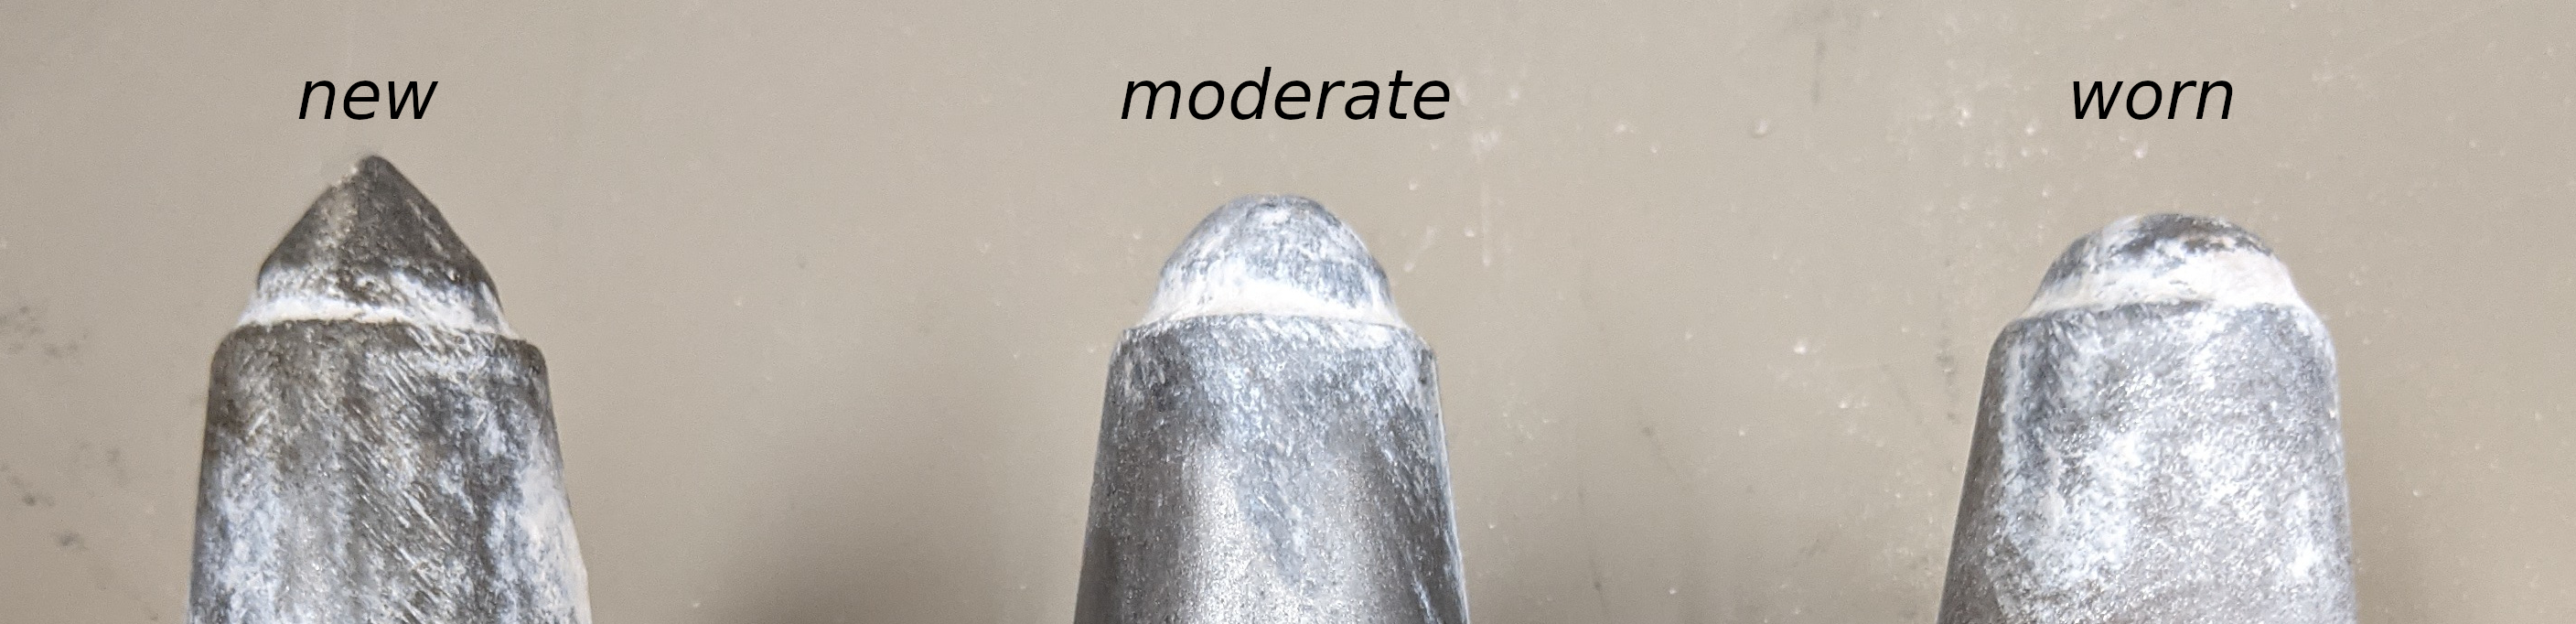
\includegraphics[width=3in]{figures/p1_media/Fig2.png}
\caption{The different pick wear levels. The \textit{new, moderate}, and \textit{worn}  pick tips
  have spherical diameters of 3.71 mm, 17.9 mm, and 27.5 mm respectively. 
 This approximates and even wear pattern. 
 The \textit{moderate} and \textit{worn} tips were artificially worn using a lathe.}
\label{fig:tips}
\end{figure}

To highlight the changes in vibrational modes, the data is transformed using
 short window fast Fourier transform preprocessing before classification.
The resulting vectors are classified into material and wear categories 
 using the support-vector machine technique. 
Data from strain gauges embedded in the linear cutting machine and our custom sensor are 
 both used on their own for classification.
Each classification system in our experiment is scored using 
 the F1 score \cite{sasaki2007truth, powers2020evaluation}.
The best performance for material and wear classification  
 yielded F1 scores around 0.85 out of 1.0 for our experiment.
Performance in tool wear classification is shown to be comparable between the custom sensor and the 
 strain gauges embedded on the linear cutting machine. For material classification, the additional
 sensitivity due to the proximity of the custom sensor to the cutting interface allows it to 
 perform better using the same algorithm.

The rest of this article is organized into sections. 
First, background information regarding material and wear classification algorithms is given along 
 with a description of the algorithm we use.
Then, the sensor design and characterization is described.
After, the procedure for the rock cutting experiment is given,
 followed by the performance results of the classification algorithm.
Finally, some discussion points and conclusions regarding the experiment and results are shared.


\subsection{Material and Wear Classification}
Material identification techniques for rock cutting can use metrics based in
 force and energy measurements, as different rock materials are known to require
 varying energy to break down \cite{teale65,klyuchnikov19}.
For tool wear classification, force or vibration feedback is commonly used in other domains such as 
 metal milling or oil drilling because changes in tool mass and geometry cause 
 the vibrational modes to shift \cite{klaic18, abu03, tao09, tao10}.
Both material and tool wear classification can be framed as a vibration classification problems.
Vibration classification lends itself towards certain standard
 signal processing and classification techniques,
 primarily with frequency domain preprocessing \cite{liu18}.

Preprocessing the input sensor data using different spectral or statistics
 based methods to improve classification results
 is popular \cite{peng11,tao09,qian10,tao10}.
For this research, the fast Fourier transform is chosen as the preprocessing technique
 as it has been shown to give good results in many domains \cite{ram09}.
Depending on the chosen kernel for the support-vector machine, data standardization
 can range from beneficial to necessary, as the kernel may be built with assumptions
 on data mean values and range.
The effects of the chosen normalization and preprocessing methods, 
 or their absence, on the classification results are explored in this work.
%For an overview of well-established spectral techniques and advice for higher
% order techniques, the reader is referred to \cite{niki87}.

The classification technique used after preprocessing is the support-vector machine (SVM)
 using the default `C-Support Vector Classification' implementation in the Python library
Scikit Learn \cite{chang11}, \cite{platt99}.
SVM has long been known to be able to classify model behaviors \cite{mukh97}.
It has also shown useful specifically in tool  monitoring \cite{sun04}.
In general, the SVM works by finding a hyperplane in the data set
 which separates the data into the prescribed categories
 then, this hyperplane can be used as a quick decision rule
 for classification of future inputs \cite{chang11}.
The advantage of the SVM is it first transforms
 the input data to a higher dimension using a kernel function which helps to separate the data.
This method has few hyperparameters and is considered
 generalizable, only needing relatively little training data to achieve good performance.

The SVM technique has few hyperparameters when compared to other 
 machine learning techniques like feed-forward or convolutional neural networks, 
 which allows it to be implemented quickly and be generalizable. 
The SVM is also typically better performing than simple techniques like k-nearest neighbors.
K-nearest neighbors is another popular and low hyperparameter technique
 for vibration classification, and it works by selecting the majority class
 of the `k' samples closest to the input in its memorized training data \cite{hu21}.
The SVM solves the classification problem in a similar way, but reduces the training data
 for computational efficiency and better sensitivity to general trends.
More advanced techniques, such as feed-forward or convolutional neural networks,
 are flexible techniques for vibration classification that work by numerically optimizing
 a series of weighted vector functions to approximate the statistical likelihood
 of a given input being from each output class based on the training data \cite{chen16}.
SVM strikes a balance between these techniques as it generally has better performance than k-nearest neighbors 
 but is not as prone to over-fitting as the feed-forward or convolutional neural network.

\subsubsection{Classification Methods}

Time-series measurements are recorded from the four channels of our custom sensor
 and the four channels of the strain gauges on the linear cutting machine.
For either sensor, we denote these measurements as $CH_x[n]$, where $x$ is the channel index 
 ranging from 1 to 4 and $n$ is the sample index ranging from 1 to $T$, the total number of measurements. 
These time-series measurements from each sensor are then chopped into small segments representing 
 short duration ($\leq 0.25$ s) windows of signal. 
These discrete vectors are preprocessed to form the feature 
 vectors to be classified by the support-vector machine. 
For an individual classification sample, the data from a particular
 channel can be denoted as $\ora{C_{kx}} = [CH_x[k], CH_x[k+1], \ldots, CH_x[k+M-1]]^\top$, where
 $k$ is the index corresponding to the start time of the sample window, $x$ is again the channel index,
 $M$ is the number of samples in the window, 
and $[\> \cdot \>]^\top$ represents the matrix transpose operation.

Both window overlap and window size are varied during our tests to observe their effects on performance. 
Increasing window overlap generates more data vectors for training and testing,
 but the resulting samples are more redundant than those generated with less overlap.
Increasing window size gives data with more features which can improve classification accuracy.
The classification rate is limited to one classification per window, 
 and windows may overlap to increase the rate.
A short window which gives acceptable performance is desired 
 for rapid classification suitable for real-time use. 

Each point in time can be assigned a class label for both material and wear. 
Only windows with contiguous labels are used in the experiment. 
Samples which are near the beginning or end of a material are discarded, 
 as they do not have a clear ground truth label and are not representative of the
 steady state cutting dynamics.
Separate classification systems are trained to identify material and wear.
For an individual classification experiment, the set of paired measurement and class data
 is split randomly into testing and training sets.
The set with the training indices is denoted in this work as $R$, while the set of testing indices is $Q$.
After being windowed and split, the feature vectors for classification via 
 support-vector machine are represented as:
\begin{align}
\ora{X_i} &= \mathcal{P}_{\theta} \Bigg( \begin{bmatrix}  \ora{C_{k1}} \\[1ex]
                              \ora{C_{k2}} \\[1ex]
                              \ora{C_{k3}} \\[1ex]
                              \ora{C_{k4}} \end{bmatrix} \Bigg) ,
\end{align}
were $\mathcal{P}$ is the preprocessing pipeline for the data and $\theta$ are the parameters fit from the
 samples in the training set.
The subscript, $i$, is the sample index and ranges from 1 to $N$, the total number of vectors
 in the data set. The specific mapping between $i$ and $k$ depends on the window parameters.
The Scikit `sklearn' library \cite{chang11, platt99} provides a convenient data structure, the Pipeline object, 
 which encapsulates these steps for consistent application and ensures that data from the 
 testing set is not used during parameter fitting. 

\begin{table}[h]
\centering
\caption{Preprocessing Pipeline Steps, $\|\cdot\|, \cdot^2$, and $\sqrt{\cdot}$ are element-wise
 absolute value, square, and square root respectively.}
\label{tab:preproc}
{\renewcommand{\arraystretch}{1.5}%
\begin{tabular}{l|l|l}
Symbol                  & Values         & Description    \\ \hline 
\multirow{2}{*}{$\mathcal{N}_\theta^1, \mathcal{N}_\theta^2$} & StandardScaler 
   & $\mathcal{N}(\ora{X_i}) = \big(\ora{X_i} - \underset{i \in R}{\mathrm{mean}} (\ora{X_{i}}) \big)/ 
                                  \underset{i \in R}{\mathrm{std}}(\ora{X_{i}})$ \\
   & None/Control   & $\mathcal{N}(\ora{X_i}) = \ora{X_i}$   \\ \hline
\multirow{3}{*}{$\mathcal{F}$}      & FFTMag        
              & $\mathcal{F}(\ora{X_i}) = [\|FFT(\ora{C_{k1}})\|,  ..., \|FFT(\ora{C_{k4}})\|]^\top$     \\
              & FFTSQ        & $\mathcal{F}(\ora{X_i}) = [FFTMag(\ora{X_i})]^2 $         \\
              & FFTSQRT       & $\mathcal{F}(\ora{X_i}) = \sqrt{FFTMag(\ora{X_i})}$      \\
              & None/Control  & $\mathcal{F}(\ora{X_i}) = \ora{X_i}$           
\end{tabular}}
\end{table}

For our experiment, the pipeline consists of the composition of three optional operations, 
 detailed in \ref{tab:preproc}, and discussed here:
\begin{align}
\mathcal{P}_\theta &= \mathcal{N}_\theta^2 \circ \mathcal{F} \circ \mathcal{N}_\theta^1
\end{align}
where $\circ$ represents the function composition operator.
The steps denoted with $\mathcal{N}$ are normalization steps which transform the input
 data to be zero mean and unit variance along each feature using the sample mean and variance
 from the training set. 
The $\mathcal{F}$ operation is the frequency based transform, and different variations of 
 the fast Fourier transform are used. 
Every combination of processing steps is used, 
 and the results are compared to determine the best methods for this application. 
Each step is also substituted with the identity function during this process as a control.

In addition to the preprocessing step, the support-vector machine also can apply a transform to the 
input data during its use. A description of the support-vector machine algorithm, 
 adapted from \cite{smola2004tutorial} is given here.
Intuitively, the support-vector machine finds a hyperplane between two sets of data. This 
is done efficiently by representing the hyperplane as a linear combination of a subset of the 
training data. These vectors from the training data are known as the support vectors.
The binary classification support-vector machine works by solving the primal problem:
\begin{align}
\min_{w, b, \xi} \quad & \frac{1}{2} \|w\| + C \sum_{i\in R} \xi_i, \\
\mathrm{s.t.} \quad & y_i [w^\top \phi(\ora{X_i}) + b] \geq 1 - \xi_i, \quad \forall i \in R.\\
                 & \xi_i \geq 0, \quad \forall i \in R.
\end{align}
where $w$ and $b$ are the vector and offset representing the decision boundary hyperplane,
$\xi_i$ are slack variables which allow for error in classification in case of an infeasible problem.
The $y_i$ are binary class labels with value -1 or 1, $C$ is a regularization parameter, 
and $\phi(\cdot)$ is an implicit function which transforms the feature vectors into a higher dimension
before separation with the hyperplane. The function $\phi(\cdot)$ is implicit because in practice 
the dual of the primal problem is solved and only the inner product of the transformed input vectors 
is computed. This is done with the `kernel trick', whereby a kernel function, $K(x,y)=<\phi(x), \phi(y)>$
is used, which is less costly to compute than the full inner product in the higher dimension. After solving
the dual problem, the decision function for an unseen sample, $\mathbf{x}$ is given by:
\begin{align}
y_{pred}(\mathbf{x}) = \mathrm{sgn} \bigg( \sum_{i \in S} \alpha_i y_i K(\ora{X_i}, \mathbf{x}) + b \bigg),
\end{align}
where the $\alpha_i$ are the new coefficients given from the dual formulation 
 and $S$ is the set of support-vector indices. 
It is noteworthy that the final decision function does not explicitly use the hyperplane
 as represented by $w$, but instead relies the offset variable $b$ 
 and dot products (through the kernel) with the training data.
To use the support-vector machine for multi-class problems, the chosen implementation
 uses a `one-vs-one' voting scheme where a binary classifier is trained for each pair of
 class combinations. The class with the lowest index and most votes is chosen as the output.

The radial basis function is a popular kernel choice, as it was one of the first to be developed.
It is similar in function and performance to using auto-correlation as the 
 implicit function \cite{kong2007autocorrelation}.
Since the radial basis function gave acceptable performance 
 and to limit the number of hyperparameters, only it is used for this study.

To test our classification system, the feature vectors are sorted into testing and training sets
using ratios of 25:75, 50:50, 75:25. Each split is done randomly, 100 times, for each combination of
preprocessing parameters. Hyperparameters for our method are window duration, window overlap ratio, and window shape.
Window duration is set to 0.05, 0.10, 0.15, 0.20 and 0.25 seconds, 
 while overlap ratio is set to 0.25, 0.50, and 0.75. 
The window shape is left as rectangular for the entire study.
Ringing effects from frequency convolution with the $\mathrm{sinc}(\cdot)$ shape of the window in the
 frequency domain will be applied consistency across samples.
Discovery of the optimal window shape would require it's own extensive hyperparameter study
 across the many popular window functions. 
To limit the scope of the study, and since adequate performance was given with the rectangular window,
 focus is given to the other hyperparameters.

The effect of the preprocessing steps or their absence is investigated for this classification system
 across the hyperparameters of window size and overlap.
Each classification setup is scored using the F1 score \cite{sasaki2007truth, powers2020evaluation} 
 which is the harmonic mean of the classifiers precision and recall:
\begin{align}
F_1 &= 2 \frac{\mathrm{precision} \cdot \mathrm{recall}}{\mathrm{precision} + \mathrm{recall}}
\end{align}
Precision is the ratio of positive classifications that are correct while recall is the ratio of 
 positive samples which are correctly identified \cite{powers2020evaluation}.
The F1 score provides a numeric value between zero and one, with one being a perfect score. 
For our multi-class problem, we train the SVM using the `balanced' strategy where classes 
 are given equal weight, regardless of class samples size, by setting regularization term, $C$,
 inversely proportional to the class frequency in the input data.
We score the classifier using `macro' averaging for the F1 score
 where the final score is the unweighted average of the F1 scores for each class.
Using this setup, the classifier is trained to give equal weight to each class type,
  regardless of population size, and classification 
 performance and is scored with a metric which also gives equal weight classifier performance
 for each class. Additionally, confusion matrices and accuracy measurements are 
 used to get a more complete sense of classifier performance.

From this study, the optimal subset of steps may be found in a verifiable way. The training and testing
 computations are performed on the Isengard supercomputer at Colorado School of Mines. Individual classifiers
can be trained on a consumer laptop in less than a minute, but to run the thousands of tests for this study
 in a batch manner, the supercomputer is more appropriate.
For each set of parameters, the mean and standard deviation of the F1 scores
 are recorded for a population of 100 experiments with different random splits of data.
Setups giving scores with large deviations or high dependence
 on the test and train ratio are suspect for overfitting to non-relevant features in the data set,
 while a low deviation with a high mean F1 score that is similar across test and train ratios can be 
 considered generalizable and useful for the target application.
To meaningfully compare distributions of scores generated for each method,
 the Welch-Satterthwaite method (Welch's t-test) is used to determine 
 if differences are significant \cite{tamhane2000statistics}

\subsubsection{Sensor Design Literature Review}
When it comes to designing a sensor for underground mining applications,
 there are several key constraints: the device must be low power, low cost,
 and highly durable. Capacitive sensors generally meet these requirements.
Sensors that are not considered directly for this study are Inertial Measurement Units (IMUs)
 or custom microelectromechanical systems (MEMS) devices due to their power consumption, cost, and fragility.
The most promising fabrication technology found during our literature review was
 capacitive load cells embedded in flexible printed circuit boards.
The sensor dynamics can be non-linear, so the collected measurements 
 are compared to those of a linear force sensor. 

Capacitive pressure sensor designs have used
 steel enclosures \cite{lee16}, film dielectric \cite{bodini18},
 and sensors made directly from flexible circuits \cite{lee08}.
Larger film dielectrics can be modeled with a general system of springs and dampers;
 however, with thin films only a few dozen $\mu$m thick, the molecular dynamics
 contribute greatly to the response \cite{willam02} and make it non-linear.
Encasing the flexible circuit element in an enclosure provides a rigid structure
 with more linear deformation, but the dielectric still affects the relationship
 between the input force and the measured capacitance.
These flexible sensors are low in cost,
 while sensors which provide more linear measurements normally employ careful
 manufacturing processes, air gap designs,
 and different signal processing techniques such as those seen in
\cite{barile19,Lu16,Zaitsev17,Prit19,Liu16}.
Sensors which use thin films with non-linear deformation must use appropriate models
 and algorithms to achieve the desired classification results.

Popular flexible dielectric materials like carbon-doped
 thermoplastic poly-urethane and silicone can exhibit non-linearity
 through hysteresis, viscoelastic effects, or measurement creep
 \cite{Shouten17,Wolter18,Dommelen20,Kisic19}.
The choice of dielectric material for a capacitive sensor will 
 influence much of its performance, so it is important that the material
 have robust properties for the expected range of conditions.
Polyimide %(also known as PI) 
is a notable flexible dielectric material and
 sensor substrate for capacitive sensors due to its high temperature range,
 solvent resistance, and low surface roughness \cite{Khan14}.
It is also easily integrated with electronic circuits boards, known as
 flexible printed circuit boards, where it serves as the substrate for conductive traces.
However, when used in a thin film, polyimide has nonlinear deformation dynamics due to the complex
 molecular interactions of the constituent polymer chains \cite{VALAVALA20071161}. 
This viscoelastic-plastic behavior can be difficult to model for a large range of input,
 with models either incorporating complicated numerical integration techniques
 \cite{dharmadasa20, li21},
 only capturing the linear viscoelastic portion for small ranges \cite{he16},
 or ignoring the unloading phase \cite{wang20}.
Thicker films generally have a greater linear range \cite{chang08} and most models
 incorporate some mix of viscoelastic and viscoplastic elements like the model seen
 in \cite{wei08}.

Other works which have used polyimide as the force or pressure sensor
 dielectric show mixed results for sensor performance.
In one study, electrospun polyimide nanofibers were used as the
 dielectric to achieve measurement repeatability and sensitivity \cite{zhu20}.
When the device was cycled from 0 to 10 \% change in nominal capacitance for 10,000 cycles,
 no noticeable measurement creep was observed.
In another study, spin coated polyimide was used, and the sensor response was much noisier
 and subject to some initial transient effects \cite{dobrzynska12}.
Another group used a FlexPCB force sensor encased in polymeric materials and
 it showed good linearity and low hysteresis for 1\% changes in capacitance \cite{Bodini19}.
These studies indicate that polyimide is a good low-cost material choice that can still give
 good performance.


\subsubsection{Sensor Design}

To design a capacitive force sensor for material and wear classification, suitable choices must be made for
 materials, geometry, and the balance between sensor accuracy and bandwidth. 
Based on the sensor design literature review, 
 a steel case with a load cell embedded in a flexible polyimide circuit board is chosen for the design. 
The steel is 303 series stainless, chosen to reduce potential for corrosion and for its
 resistance to fatigue.
The steel case is made by chemical etching of 0.036 inch steel plates. 
A channel of 0.018 inch depth is formed on one plate and the two are laser welded together after
 a steel shim and the sensing membrane have been put in place.
As noted in the prior section, polyimide is chosen for the sensing membrane for its
 wide range of operating conditions and robust properties.
The sensor case geometry is largely determined by the target tooling, but must still be tuned to the operational
 requirements of the sensor. 
Likewise, the balance between sensor accuracy and bandwidth must be tuned to achieve the desired results.

To tune the case geometry for the desired stiffness, appropriate values must be chosen for the
 thickness and height of the side walls.
These values are shown as $\mathbf{h}, \mathbf{w_1}$ and $ \mathbf{w_2}$ in Fig.~\ref{fig:sensecut}.
The donut shaped sensor has a center filled with viscous polyimide. 
The thickness and height of the side walls chiefly determines the spring constant of the sensor.
The polyimide is much more compliant than the surrounding steel, so the overall case deformation is not 
 influenced by its deformation in a significant way.
However, the capacitive cells are directly embedded in the polyimide, so the measurement is greatly 
 influenced by its deformation.


\begin{figure}[t!]
\centering
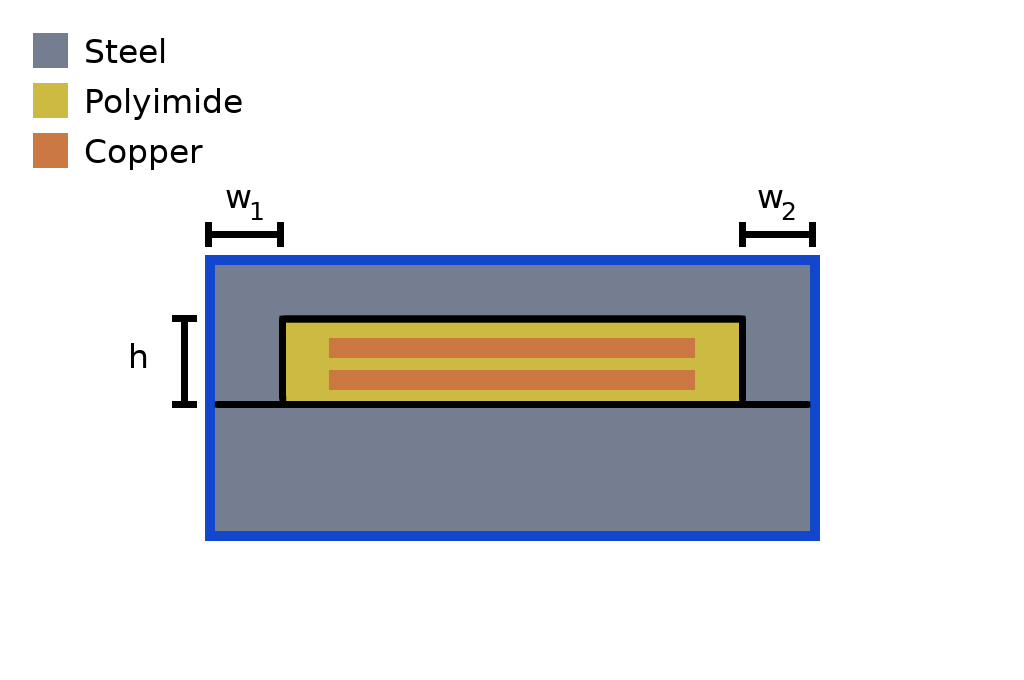
\includegraphics[width=3in]{figures/p1_media/Fig3.png}
% sensor geometry cutaway
\caption{
A cutaway of the sensor with the geometric parameters shown. The dimensions of the walls
 may be tuned to give the sensor the appropriate stiffness. The thickness of the top and bottom plates
 do not significantly influence the overall stiffness of the device.
}
\label{fig:sensecut}
\end{figure}


The sensor is designed for a maximum expected force of 200 kN. 
This provides some margin above the expected forces, which can be in excess of 100 kN for hard rocks.
The sensor case is tuned to have around 10\% strain at maximum load, in this way material fatigue can be 
 mitigated and the measured capacitance should be close to linear with dielectric deformation.
The thickness and height of the side walls, $\mathbf{h}, \mathbf{w_1}$ and $\mathbf{w_2}$
 are set to about two and a half millimeters.
The deformation of the steel case is expected to be mostly linear within this range of deformation.

The balance between sensor accuracy and bandwidth is determined by the range of deformation of the sensor
 as well as the capacitance and resonant frequency of the sensing circuit.
In general, larger capacitance values will provide greater accuracy at the cost of sensor bandwidth.
For the chosen hardware, the effective number of bits for the measurement 
 is proportional to the square of the measurement time. 
Larger capacitances take longer to settle but can make more accurate measurements.

Given the tool geometry, four cells are placed in the donut: two large and two small.
For our parallel plate design, it is important that the electrodes receive even loading,
 otherwise the parallel plate approximation is no longer valid.
The large cells are designed for a nominal capacitance of 541 pF and 
 the small cells are designed for a nominal capacitance of 412 pF.
All four pads occupy about $50^\circ$ and are spaced evenly around the donut.
The larger cells have about 30\% greater area.

Since we are focused on high-frequency vibration classification, 
 sensor bandwidth is maximized while still 
 providing sufficient resolution and accuracy for classification.
At a rate of 400 samples per channel per second, and using a gain of 4, 
 the embedded system is able to provide 128 levels for up to a 25\% change in capacitance.
At 10\% max expected deformation, the max expected change in capacitance is also about 10\%.
The true deformation of the polyimide around the electrodes is nonlinear and must be characterized to 
 make informed decisions with the resulting measurements.
 

\subsubsection{Sensor Characterization}

The sensor was characterized using load frame testing.
Five different load rates were applied to three separate sensors to achieve a max force of 200 kN 
 momentarily before ramping back down at an equal rate. 
Linear sensors show symmetric behavior for such a test, 
 but the sensor measurements for this test, shown in Fig.~\ref{fig:triangleload}, 
 reveal that our sensor exhibits hysteresis and rate dependence for these loads.
These effects can be expected from the previous literature regarding polyimide deformation
\cite{Khan14, VALAVALA20071161, dharmadasa20, li21, he16, wang20, chang08, wei08, zhu20, dobrzynska12, Bodini19},
 and they obscure the effect of the average force on the measurement.
It can be seen that, as the loading rate increases, the traces converge.
This implies that the sensor can still be used to detect the changes in the high frequency components 
 of the response that are useful for vibration classification.
The overall deformation of the sensor case during these same loads is shown in Fig.~\ref{fig:casedeformation},
 and the deformation is linear. 
This confirms that the nonlinear deformation is happening in the polyimide
 and suggests that this case could be used to house other sensing technologies
 that can transduce displacement to electrical signals.

\begin{figure}[t!]
\centering
\centerline{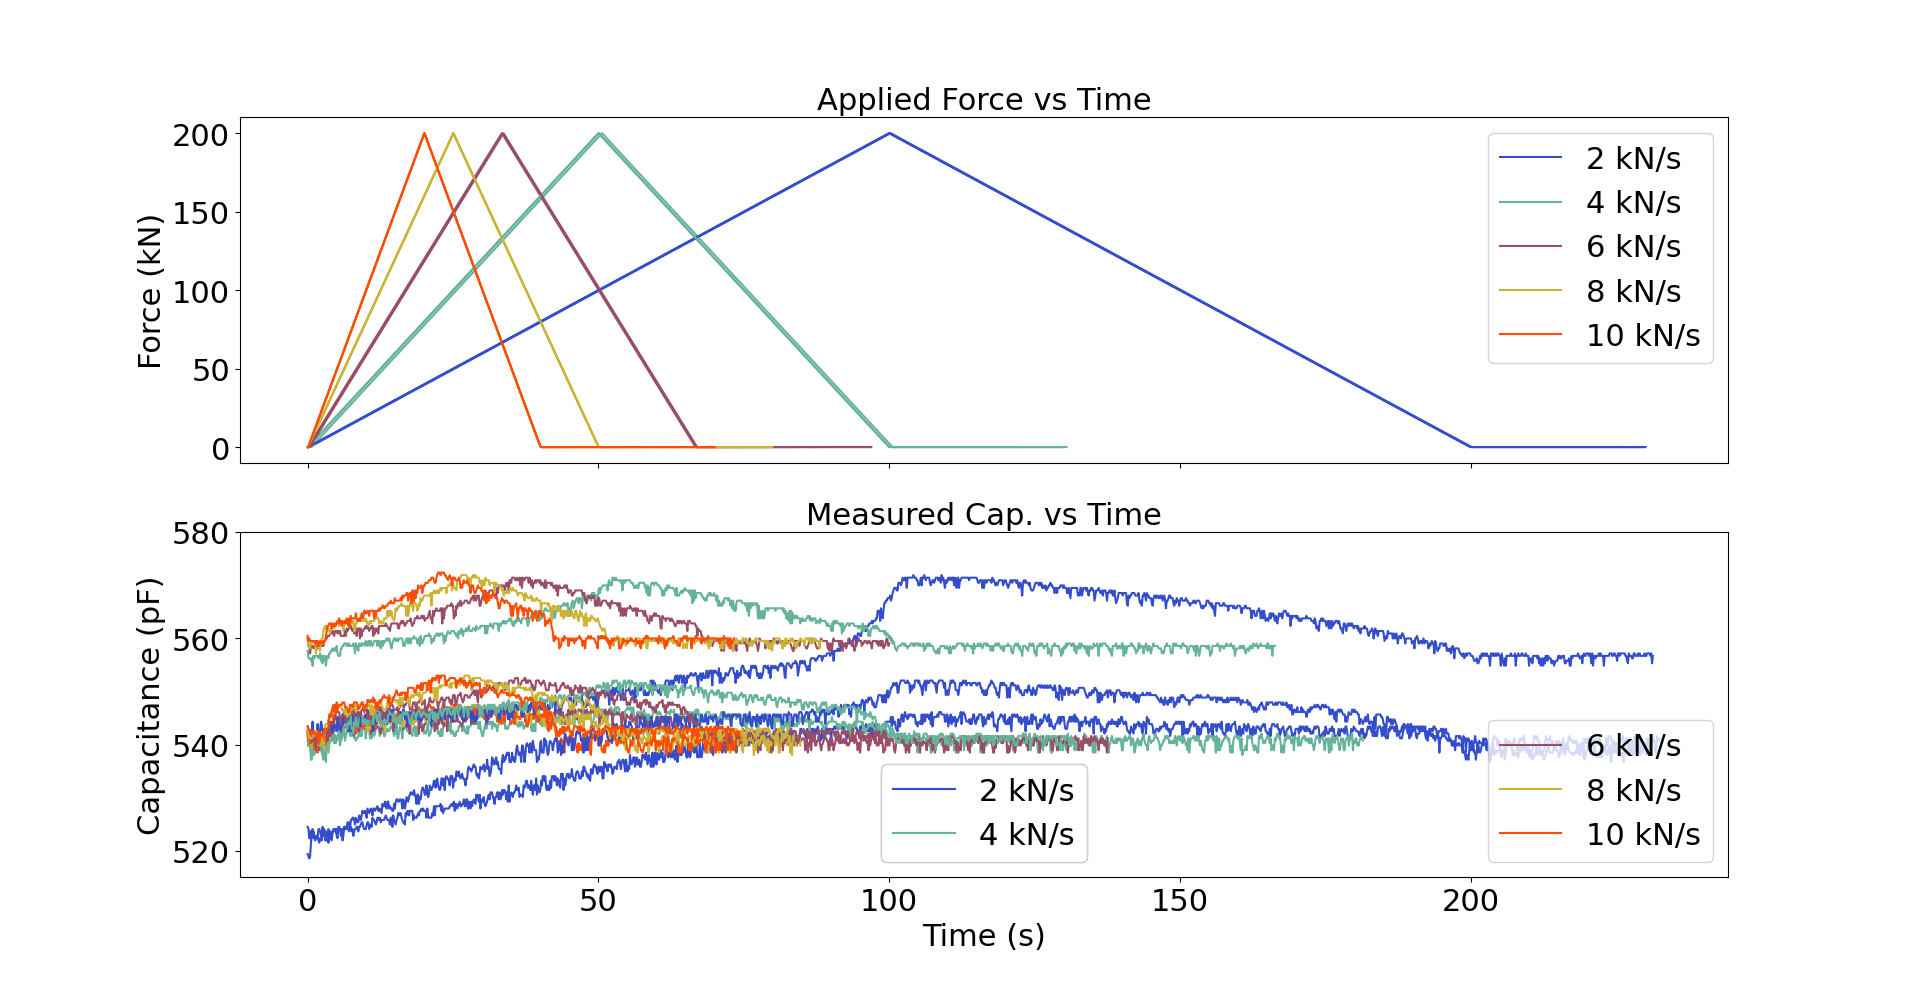
\includegraphics[width=5.5in]{figures/p1_media/Fig4.png}}
% sensor triangular tests
\caption{
The triangular load profiles and the resulting measurements from the sensor. 
The sensor response is not symmetric and therefore non-linear.
Lower load rates cause greater changes in displacement, which is consistent with previous studies for 
 thin film polyimide. 
}
\label{fig:triangleload}
\end{figure}

\begin{figure}[t!]
\centering
\centerline{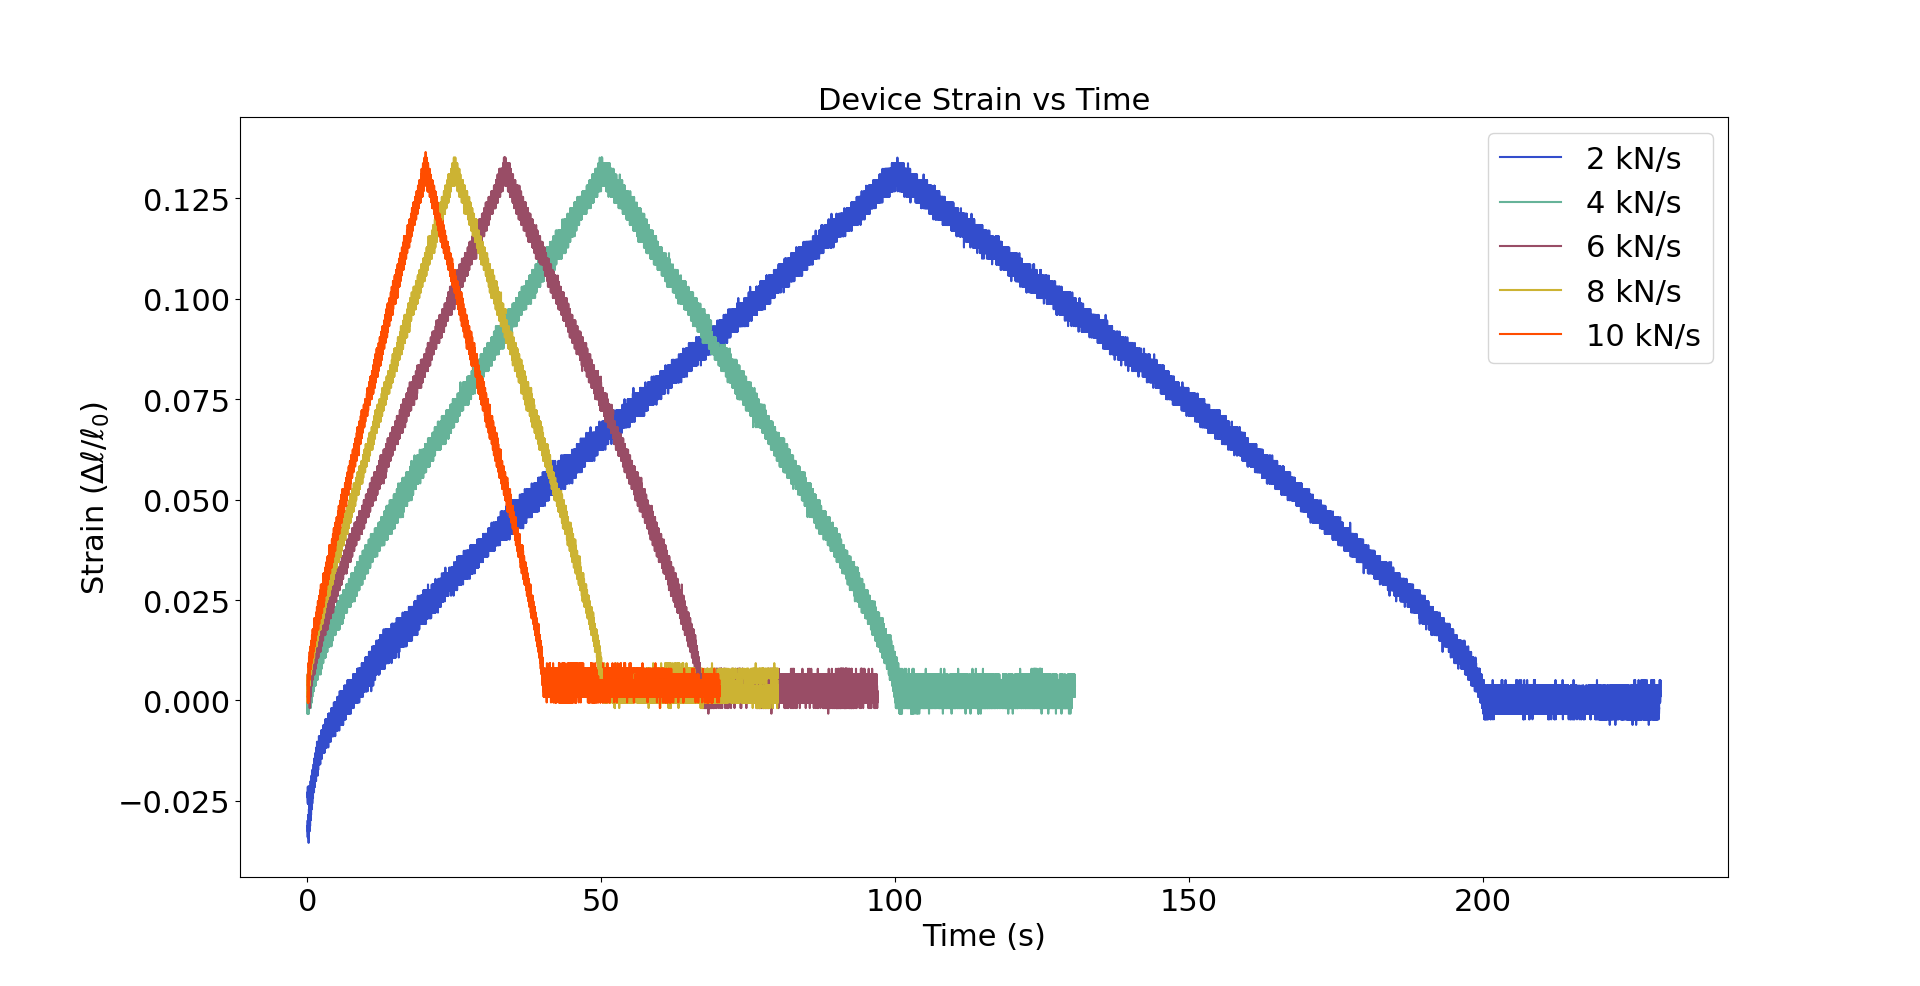
\includegraphics[width=5.5in]{figures/p1_media/Fig5.png}}
% sensor case deformation
\caption{
The case deformation during the load frame tests. The case deformation is symmetric for the 
 loading and unloading phases, it also has a consistent slope for force over displacement.
This means the case has approximately linear deformation for these load profiles.
}
\label{fig:casedeformation}
\end{figure}

\subsection{Rock Cutting Experiment}

To test the sensor for \textit{in-situ} force signature capture, rock cutting experiments
 were performed using the Linear Cutting Machine in the Earth Mechanics Institute at the 
 Colorado School of Mines.
A limestone sample cast in concrete was cut using a conical pick
 on the instrumented block. 
Time series measurements were made with the custom sensor as well as
 strain gauges integrated with the test equipment. 
The measurements were cut into small intervals and used with the classification 
 algorithms to build separate material and wear classifiers


To capture the capacitive measurements, a capacitance to digital converter made by
Texas Instruments is used: the FDC2114. This device interfaces with a generic 
microcontroller over I2C, a popular circuit to circuit interface. The software
used on the microcontroller is available on Github as well as the data-acquisition software
which is ran on the host computer to collect the measurements.
The software that performs the classification experiment described in the previous section is also available.
The microcontroller code is available here:  \url{https://github.com/Fworg64/DAQuery}.
The data-acquisition code is available here: \url{https://github.com/Fworg64/reDAQ}.
The machine learning and classification code is available here: 
\url{https://github.com/Fworg64/limestone_experiment}.


The Linear Cutting Machine, shown in Fig.~\ref{fig:lcmaction},
 uses hydraulic actuators to drag the sample against the cutting tool.
A cutting speed of 10 inches per second was used, which is relatively slow 
 compared to the cutting speeds used in the field.
The integrated strain gauges measure forces at a rate of 537.6 samples per second. 
The custom load cell makes measurements at a rate of 400 samples per second.
The measurements from each sensor were recorded for use in the classification experiments.
For applications with greater cutting speed and more materials, 
 consider that rock fracture is largely static and machine vibration is dynamic.
The frequency domain features associated with tool wear should scale with cutting speed 
 and depend largely on the machine's natural modes, 
 while those associated with material breakdown occur at much higher frequencies.

\begin{figure}[t!]
\centering
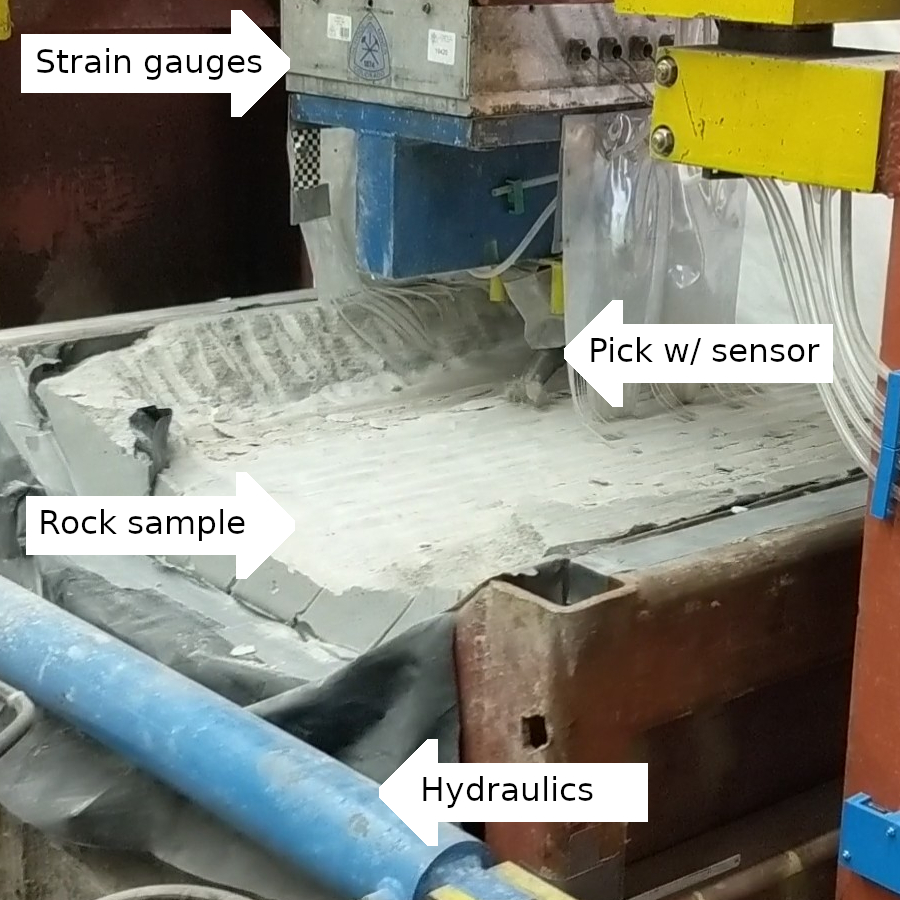
\includegraphics[width=3in]{figures/p1_media/Fig6.jpg}
%LCM figure
\caption{
The Linear Cutting Machine in action. Hydraulic actuators push the sample into the cutting tool
while the custom sensor and the embedded strain gauges record measurements. 
The tool is normally surrounded by the plastic curtain to aid in capturing dust for a 
 simultaneous study of the effect of tool wear on dust generation.
}
\label{fig:lcmaction}
\end{figure}

\subsection{Classification Results}

% Features after pre-processing
Using the method outlined in Section 2, the collected data is used to train and test
 the classification algorithm.
The capacitive sensor data gave results similar to the linear sensor in tool wear classification.
For material classification, the capacitive sensor generally performed better.
The distribution of feature vectors, before being processed with the support-vector machine kernel,
 are shown for both sensors by material in Fig.~\ref{fig:matsigs} and by tool wear in Fig.~\ref{fig:wearsigs}. 
From these distributions, it can be seen that the capacitive sensor is much more sensitive to the higher frequency 
 components of the interaction forces. 
This is likely a result of its closer proximity to the cutting interface.
Typical measurements from cutting experiments are shown in Fig.~\ref{fig:cutforces}. 

% Distributions of scores by window size, significance
For each sensor and application, five window sizes were tested. 
This gives ten pairs for comparison among each group of five, 
 so we choose $p<0.01$ as statistically significant for differences in performance.
The distributions of F1 scores for the classifiers with different window sizes are shown in Fig.~\ref{fig:windows}.
For tool wear classification, performance was similar for all window sizes for both sensors.
For material classification, the capacitive sensor gave measurements which could be more reliably classified.
The differences in performance across window sizes are significant for material classification with either sensor.

% Results 
Classification scores broken down by technique for the 0.2 second window size are shown in Fig.~\ref{fig:methods}.
Trends in relative method performance were the same across window sizes.
It was found that normalization after transformation, and not before, gave the best performance for 
 the Fourier based methods.
Also, the normalized time-series data with the SVM gave the best performance for 
 tool wear classification in both the strain gauge and capacitive sensor cases.
For material classification with the strain gauges, most methods gave similar performance.
Normalization improved classification performance in nearly all categories.

Overall, tool wear in our data was classified with greater accuracy than material type. 
For tool wear, the normalized time domain data gave better classification results than
 the frequency data.
For material type, only the capacitive sensor gave results that would be useful. 
The strain gauge data was classified with about 50\% accuracy by the classifier.
With the capacitive sensor classification of material type, 
performance using the frequency based data gave slightly better accuracy than the time
domain data.

When using only 25\% of the data for training, the classifier was still able to perform
reliably using the capacitive sensor data. 
This shows that performance was not very dependent on the test and train ratio.
F1 scores with standard deviations are given for the best setup for each application 
 at different test and train ratios in Table~\ref{tab:fourscores}.
The scores do not change by a large magnitude, which indicates that 
 the classifier is general and should perform well for larger data sets.

Individual confusion matrices are given for the 25:75 test and train ratio for 
 material classification in Table~\ref{tab:mat_conf} 
 and for tool wear classification in Table~\ref{tab:wear_conf}.
For these confusion matrices, rows represent the true class for the samples and columns represent the 
 predicted class. Diagonal entries represent correct classifications, 
 and each column is normalized to the number of predictions made of that class.
The strain gauge material classifier has poor precision for concrete samples, 
 as many of its concrete predictions are actually limestone samples. 
The F1 score is sensitive to this, and it is reflected in the much lower score.
The accuracy of the strain gauge material classifier is around 80\%, which 
 is still useful. 
The accuracy of the capacitive sensor material classifier is higher, above 95\%.
This highlights the importance of using multiple metrics to 
 accurately assess classifier performance.

\begin{figure}[t!]
\centering
\centerline{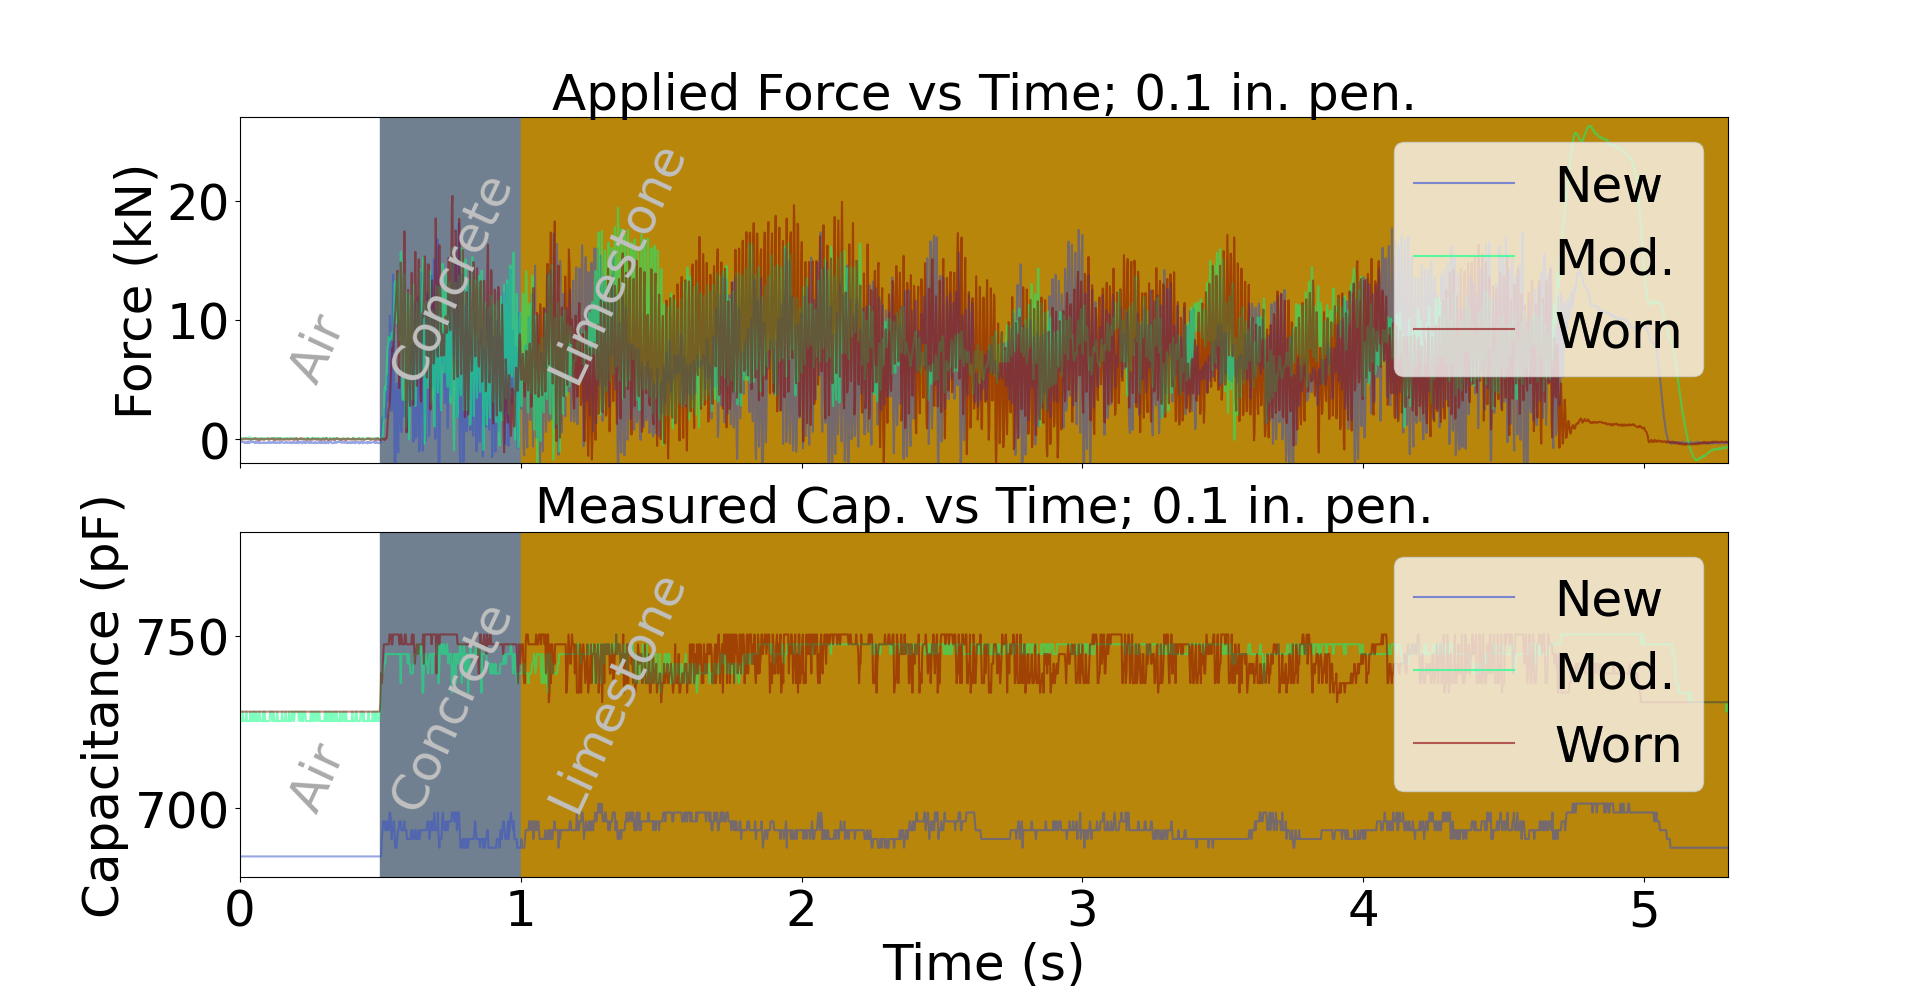
\includegraphics[width=5.5in]{figures/p1_media/Fig7.png}}
%cutting measurements
\caption{
Measurements for typical rock cuts with different tool wear levels. The measurements from the 
linear sensors are shown in the top graph while the measurements from the custom sensor are shown below.
}
\label{fig:cutforces}
\end{figure}

\begin{figure}[t!]
\centering
\centerline{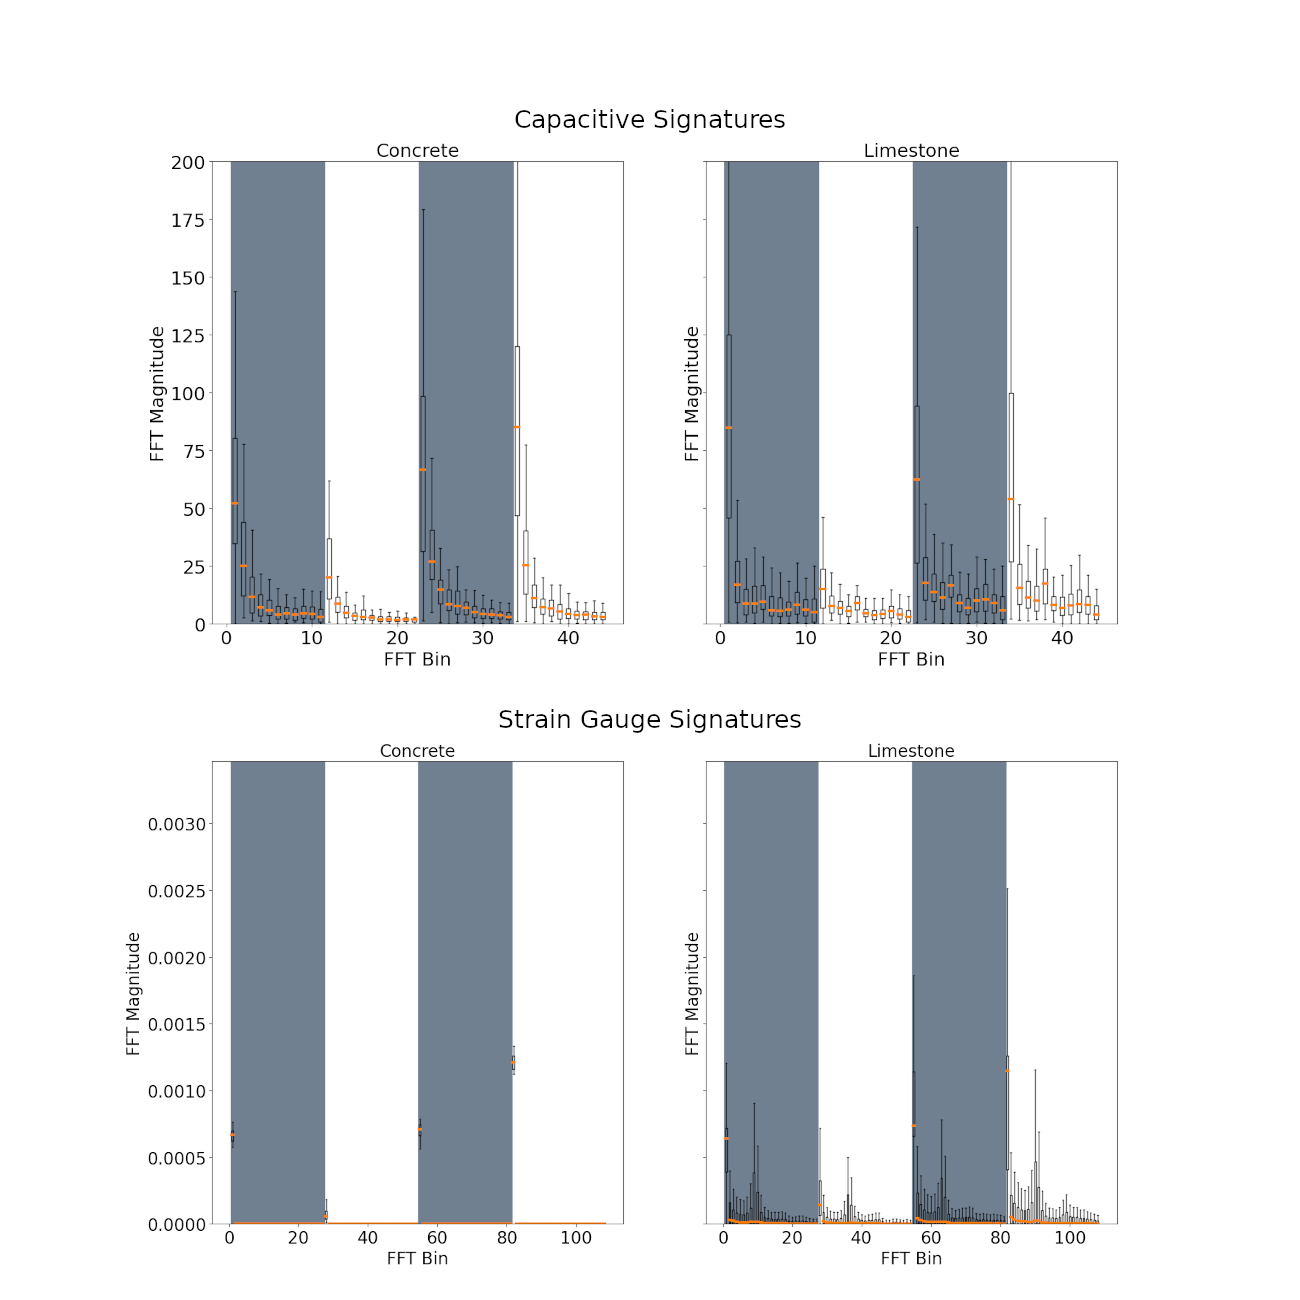
\includegraphics[width=5.5in]{figures/p1_media/Fig8.png}}
%material sigs
\caption{
The frequency signature distributions collected from the custom sensor organized by material.
The concrete material shows exponential decay after each primary mode, while the limestone 
 has a more varied response. These differences can be used for classification of the signals by material.
}
\label{fig:matsigs}
\end{figure}

\begin{figure}[t!]
\centering
\centerline{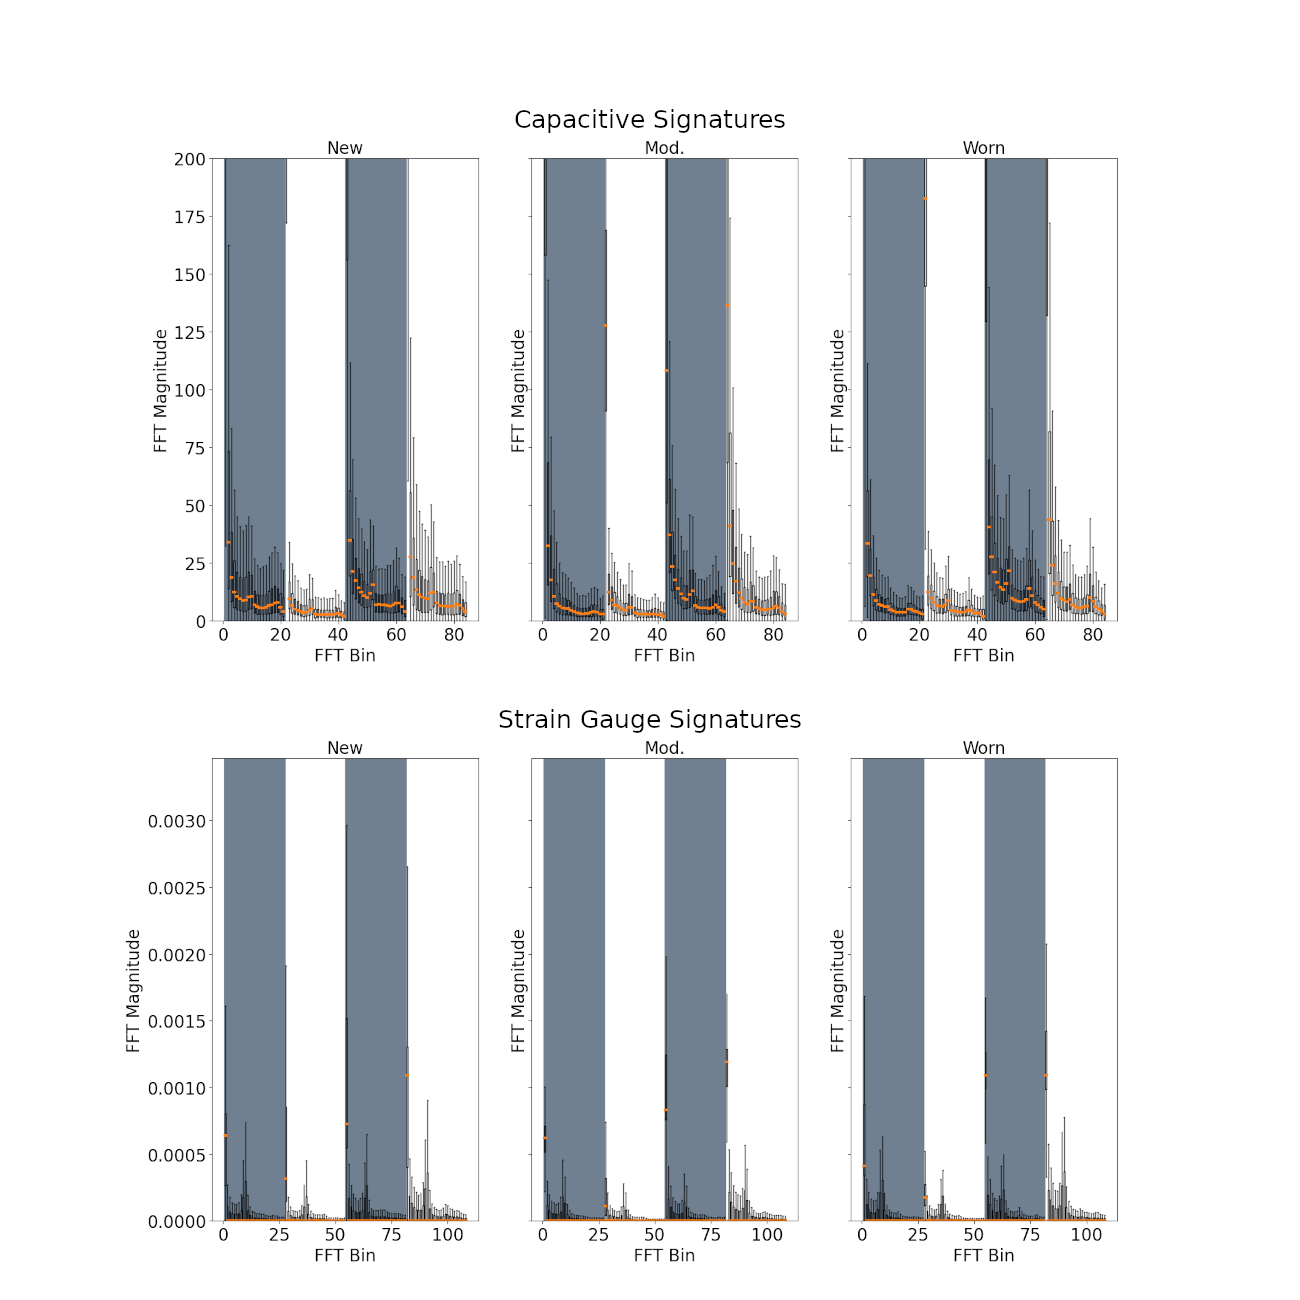
\includegraphics[width=5.5in]{figures/p1_media/Fig9.png}}
%wear sigs
\caption{
The frequency signature distributions collected from the custom sensor organized by tool wear.
The New tool has a distinct response compared to the Moderate and Worn tools, and the 
 energy in the higher modes generally increases with wear.
These differences can be used for classification of the signals by tool wear.
}
\label{fig:wearsigs}
\end{figure}

\begin{figure}[t!]
\centering
\centerline{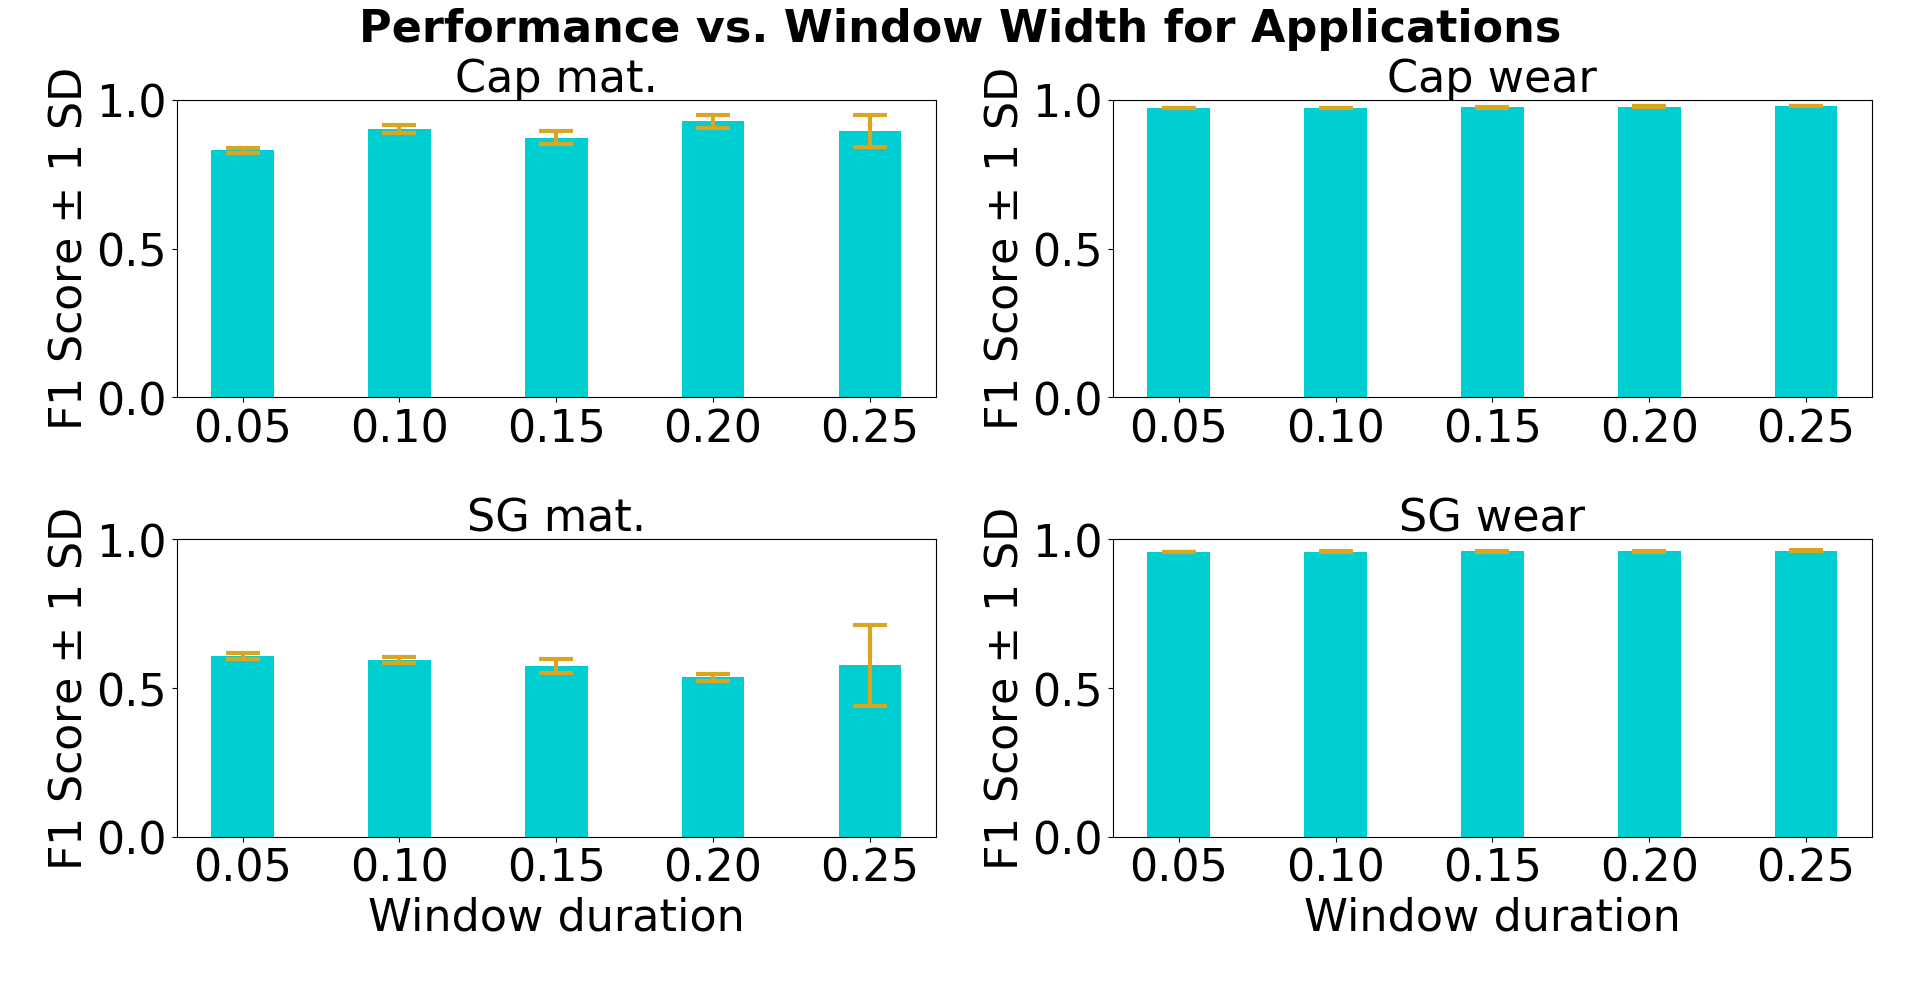
\includegraphics[width=5.5in]{figures/p1_media/Fig10.png}}
%Windows
\caption{
Bar chart with error bars for F1 score distributions by window size. For tool wear, both
 sensors were able to provide sufficient data for very accurate classification.
For material classification, the capacitive sensor generally performed better than the
 strain gauge sensor. Some of the differences in performance are significant within the 
 application and sensor combinations, but in general performance was similar across window sizes.
}
\label{fig:windows}
\end{figure}

\begin{figure}[t!]
\centering
\centerline{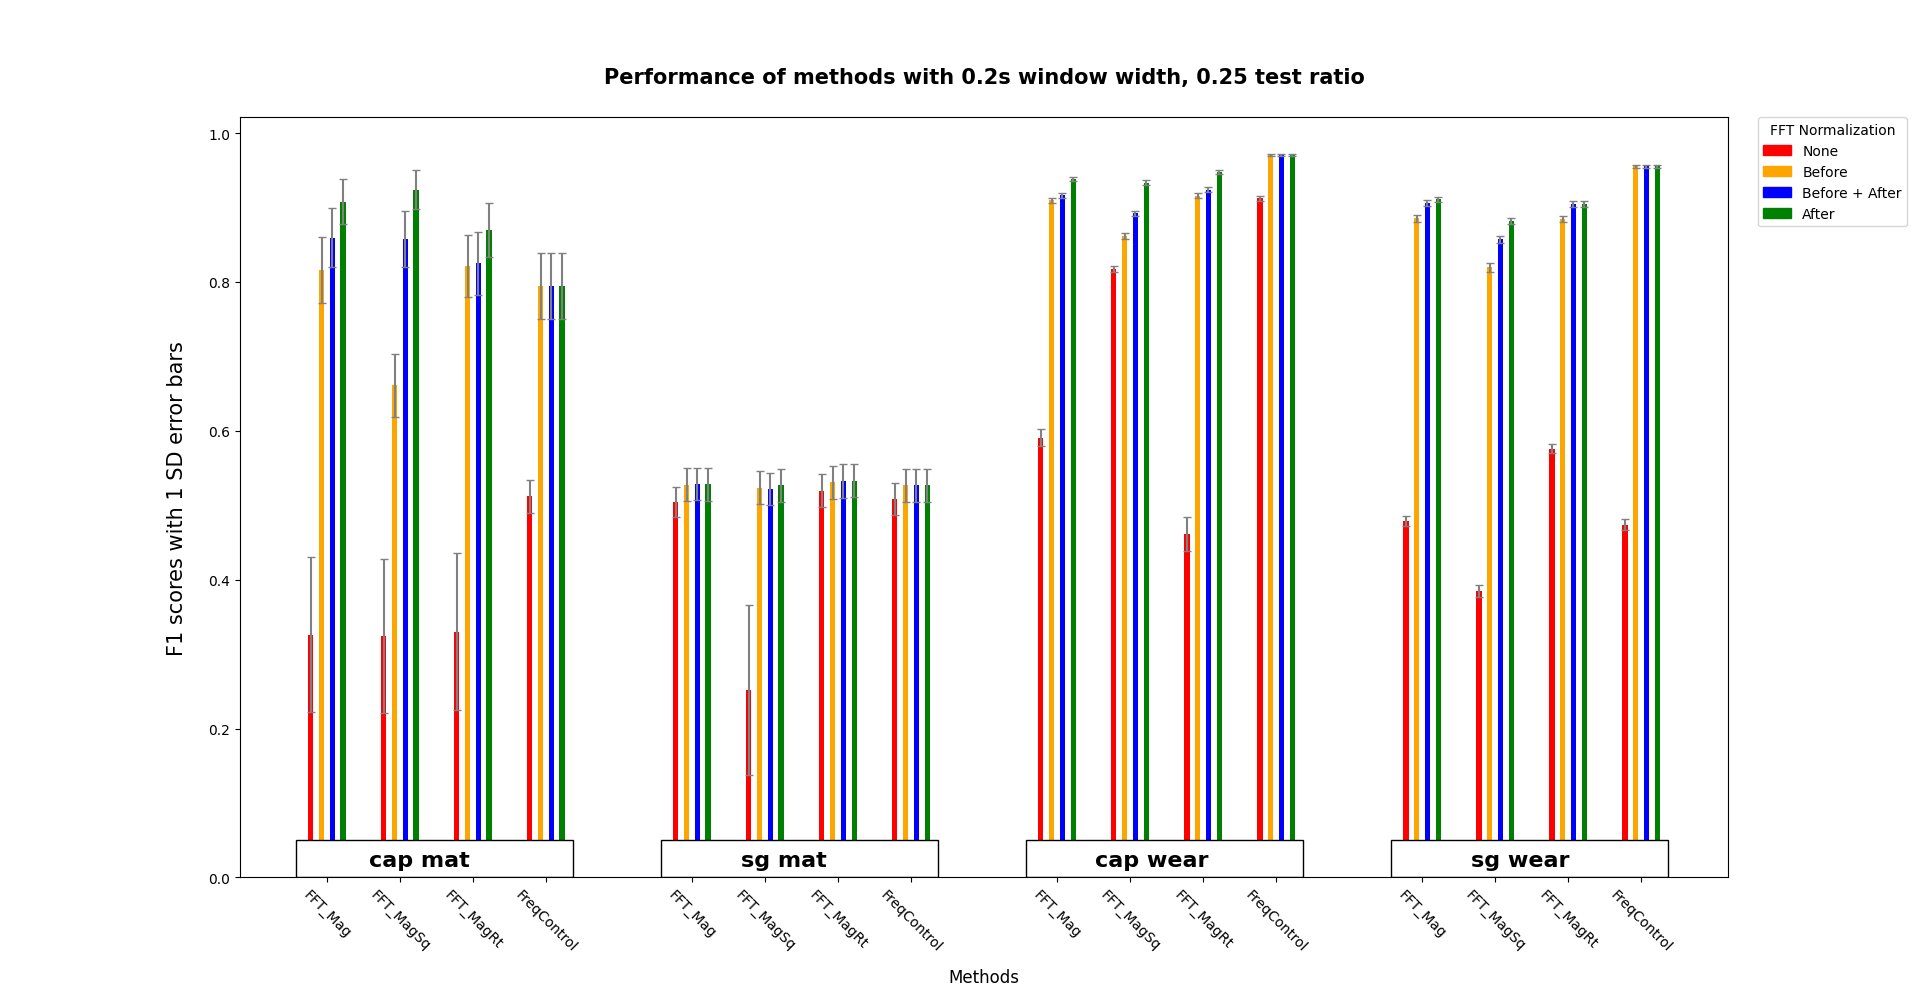
\includegraphics[width=5.5in]{figures/p1_media/Fig11.png}}
%Methods
\caption{
Performance of different preprocessing methods for each application. In general, normalization
 after transformation proved most effective for the frequency based techniques. 
 Using the normalized time domain data was most effective for tool wear classification.
}
\label{fig:methods}
\end{figure}

% Please add the following required packages to your document preamble:
% \usepackage{multirow}
\begin{table}[]
\caption{Scoring metric and test/train ratios for each application}
\begin{tabular}{lll|lll}
\multicolumn{3}{l|}{F1 Scores (mean $\pm$ std. dev., 100 trials)}                                                        & \multicolumn{3}{l}{Test and Train Ratio} \\ \hline
Application                                     & Sensor                    & Best Config.                
   & 25:75      & 50:50      & 75:25      \\ \hline
\multicolumn{1}{l|}{\multirow{2}{*}{Tool Wear}} & \multicolumn{1}{l|}{Cap.} & Time Domain 
   & $0.971 \pm  0.003$   & $0.965 \pm 0.003$ & $0.950 \pm 0.004$  \\ \cline{2-6} 
\multicolumn{1}{l|}{}                           & \multicolumn{1}{l|}{SG}   & Time Domain 
   & $0.955 \pm 0.005$    & $0.947 \pm 0.004$ & $0.934 \pm 0.004$  \\ \hline
\multicolumn{1}{l|}{\multirow{2}{*}{Material}}  & \multicolumn{1}{l|}{Cap.} & FFTMagSq 
   & $0.924 \pm 0.053$    & $0.902 \pm 0.044$ & $0.831 \pm 0.085$  \\ \cline{2-6} 
\multicolumn{1}{l|}{}                           & \multicolumn{1}{l|}{SG}   & FFTMagRt 
   & $0.533 \pm 0.045$    & $0.536 \pm 0.026$ & $0.534 \pm 0.016$  
\end{tabular}
\label{tab:fourscores}
\end{table}

\begin{table}[h]
\centering
\caption{Confusion Matrix for Material Classifier; Normalized by prediction \newline
         New Picks, 0.3 in Penetration, 0.2s Window, 50:50 test and train, PSD w/ post norm.}
\begin{tabular}{l|ll|ll}
\% Pred.   & \multicolumn{2}{l|}{Strain Gauge Prediction}                & \multicolumn{2}{l}{Cap. Prediction}                          \\ \hline
True Class & \multicolumn{1}{l|}{Concrete} & \multicolumn{1}{l|}{Limestone} & \multicolumn{1}{l|}{Concrete} & \multicolumn{1}{l|}{Limestone} \\ \hline
Concrete   & 0.117& 0.000                     &  0.923                    & 0.013\\
Limestone  & 0.883& 1.000                     &  0.077                    & 0.987
\end{tabular}
\label{tab:mat_conf}
\end{table}

\begin{table}[h]
\centering
\caption{Confusion Matrix for Tool Wear Classifier; Normalized by prediction \newline
         All Materials, All Penetrations, 0.2s Window, 50:50 test and train, Normalized Time Domain Data}
\begin{tabular}{l|lll|lll}
\% Pred.   & \multicolumn{3}{l|}{Strain Gauge Prediction}                & \multicolumn{3}{l}{Cap. Prediction}                          \\ \hline
True Class & \multicolumn{1}{l|}{New} & \multicolumn{1}{l|}{Mod.} & Worn & \multicolumn{1}{l|}{New.} & \multicolumn{1}{l|}{Mod.} & Worn \\ \hline
New         & 0.983   & 0.105  & 0.000      & 1.000     & 0.000     & 0.000 \\
Mod.        & 0.016   & 0.893  & 0.015      & 0.000     & 0.980     & 0.082 \\
Worn        & 0.001   & 0.002  & 0.985      & 0.000     & 0.020     & 0.918
\end{tabular}
\label{tab:wear_conf}
\end{table}

\subsection{Discussion}

Our sensor, as used in our experiment, shows promise as a method to objectively assess material type and tool wear.
Under laboratory conditions, the sensor and classification scheme was able to detect differences in 
mode excitation caused by different materials and tool wears. For our experiment, the materials chosen were
limestone and concrete. These materials are both much stronger than coal, but our experiment shows that they
excite distinct modes in our cutting equipment. For tool wear, it is known that more worn tools can
require several times the force to cut when compared to a new tool. The modes that are excited in the
machine also change based on the changing tool geometry. For the target application of coal mining,
coal is known to be much weaker than the material in which it is embedded, e.g. limestone. 
So, if our sensor is able to differentiate between concrete and limestone,
 it is postulated that it could differentiate between limestone and coal, which is much softer.

Using the Support-Vector Machine, the hyperplane between the measured datasets is found. 
This means that for a given input of discrete frequency or time samples, each value is 
 multiplied by a coefficient and then combined to a single value, similar to a digital filter. 
The Support-Vector Machine has few hyperparameters, and the chosen measurements 
 are shown to contain modal shifts that correspond with the categories of interest. 
The fundamental change in signal occurs as a mode distribution shift.
This is readily detected by the Support-Vector machine.

To adapt our sensor to the target application, 
the target machine would need to be characterized in terms of dynamic modes.
The sampling rate of the sensor system will need to be sufficiently higher than
the primary modes of the target tooling, otherwise the measurements could be subject to aliasing.
So long as the sampling rate at least satisfies the Nyquist criterion for the tool primary modes,
aliasing should be minimized due to the high frequency attenuation caused by massive mechanical systems.
Further, the viscous nature of the polyimide sensor provides even more damping, reducing the possibility
for aliasing at the physical level.

Additional sensor designs such as an air-gap capacitive displacement sensor should also be investigated,
 as they could likely achieve more linear measurements at the cost of sensitivity.
Development of a suitable power source and communication system must still be considered for this
application.
Other technologies such as acoustic sensors also show promise for material and wear classification,
 as they have been used with success in other domains and acoustic information is one of the primary 
 feedback mechanisms currently employed by operators. A load cell based technology would likely
be less susceptible to outside interference by unrelated signal when compared to an acoustic sensor,
as it is closer to the mining interface and collects signal from a more narrow bandwidth.

\subsection{Conclusion}

A sensor suitable for \textit{in-situ} sensing of vibration signatures for material and wear classification
 was developed and tested for underground mining using conical picks. 
The classification accuracy achieved in the laboratory tests indicates that this is a promising 
 technology for this application.
The capacitive sensing design is low cost and low power due to its flexible circuit design.
This technology could assist operators in material and wear classification by providing an objective
 measurement without requiring the operators to enter known hazardous regions near the machine and mining interface.

The capacitive load cell, to the authors knowledge, has not been used publicly for conical picks in 
rock cutting applications. This is a relatively new sensor technology that has been enabled by the 
steady advancement of capacitive sensor research over the last few decades.
Existing solutions for hazard monitoring in underground coal mining primarily identify problems
after they begin. 
Existing research in improving operator performance
and safety has included acoustic classification systems and algorithms, strain-gauge based solutions, 
and piezo-electric sensors.
By shifting the paradigm to predictive maintenance and more responsive control,
 operators are enabled to be safer and more efficient. 

\subsection{Disclosures}

\subsubsection{Conflicts of interests}
On behalf of all authors, the corresponding author states that there is no conflict of interest. 
This work was funded by NIOSH Contract 75D30119C05413, ``IMPROVING HEALTH AND SAFETY OF MINING OPERATIONS
THROUGH DEVELOPMENT OF THE SMART BIT CONCEPT FOR AUTOMATION OF MECHANICAL ROCK EXCAVATION
 UNITS AND DUST MITIGATION''.

%\subsection{References}
%\bibliography{supporting-files/sources_flexpcb}% common bib file

